\documentclass[a4paper,12pt]{article}

\usepackage[utf8]{inputenc}
\usepackage[T1]{fontenc}
\usepackage[spanish]{babel}
\usepackage{amsmath, amssymb}
\usepackage{graphicx}
\usepackage{float}
\usepackage{hyperref}
\usepackage{listings}
\usepackage{xcolor}

% Define colors for syntax highlighting
\definecolor{codegreen}{rgb}{0,0.6,0}
\definecolor{codegray}{rgb}{0.5,0.5,0.5}
\definecolor{codepurple}{rgb}{0.58,0,0.82}
\definecolor{backcolour}{rgb}{0.95,0.95,0.92}

\lstdefinestyle{pythonstyle}{
    language=Python,
    backgroundcolor=\color{backcolour},
    commentstyle=\color{codegreen},
    keywordstyle=\color{magenta},
    numberstyle=\tiny\color{codegray},
    stringstyle=\color{codepurple},
    basicstyle=\ttfamily\footnotesize,
    breakatwhitespace=false,
    breaklines=true,
    captionpos=b,
    keepspaces=true,
    numbers=left,
    numbersep=5pt,
    showspaces=false,
    showstringspaces=false,
    showtabs=false,
    tabsize=4
}
\lstset{style=pythonstyle}



\begin{document}

{\centering \textsf{TFG Pepe}\par}

\vspace{0.5in}

{\huge Lunes 2 de marzo de 2026}

\vspace{0.5in}

¡Hola José! No hice todo lo que hablamos la semana pasada, pero pienso que lo que hice da para vernos.

\tableofcontents

\section{Sobre la semana pasada}

Implementé el \emph{weight sharing} de los diccionarios de ISTA y el truco para tener más resolución en los mapas de activación.

\subsection{\emph{Weight sharing} del diccionario}

Lo cierto es que los entrenamientos son mucho más rápidos, los modelos más pequeños y [comentar diferencias].

% plot los 4 runs

% plot de sparsity y tal

\subsection{Mapas de activación}

Ahora que son más resolutivos vemos que: las primeras cabezas implementan derivadas primeras de $x$ e $y$ y las atenciones responden a información de ese token y ya, pero en capas más profundas responden a la imagen como un todo (por eso vemos que los tokens de las cabezas finales son más o menos parecidos entre sí, porque la información que portan ya no tiene tanto que ver con el parche de la imagen sino con la tarea (\emph{¿hay vena en el píxel central de la imagen?})).


\subsection{Me queda pendiente}

\begin{itemize}
    \item Mezclar órdenes inferencia / entrenamiento.
    \item Desacoplar \emph{positional embeddings}.
\end{itemize}


\section{Sobre el coste de la atención}

Esta sección discute una posibilidad que no implementé. Es decir, más elucubración, pero bueno, espero que no te moleste.

La semana pasada me recomendaste la lectura de DeepSeek por lo de la mezcla de expertos. Me lo imprimí. Como algo ya conocía de eso por Técnicas Avanzadas del Procesamiento del Lenguaje Natural, y sabía más o menos cómo era el truco, no me motivaba mucho\ldots\ Busqué y encontré un artículo estupendo: el Linformer \url{https://arxiv.org/pdf/2006.04768}. Su truco es:

Imagínate una atención genérica $\text{softmax}(Q'K/\sqrt{d})V$. Tú me venías alertando de la complejidad $\mathcal{O}(n^2)$ porque $Q'$ es $n \times d$; entonces lo que va dentro del softmax es $n \times n$ y luego si multiplicas por $V$ ahí está el tema. Evidentemente tú y yo sabemos de primero de álgebra que lo que va dentro del softmax no puede ser de rango mayor que $d$. Esencialmente el artículo demuestra que el softmax no cambia eso. ¿A dónde quiero llegar? Si sabemos que estamos haciendo un producto de matrices grandes de rango bajo, de buena manera podemos hacer un producto de matrices pequeñas de rango completo sin perder información; de forma natural:
\[
    \text{softmax}(Q'KE/\sqrt{d})FV
\]
donde $E$ y $F$ son las matrices de reducción y ampliación de dimensionalidad respectivamente.


\section{Necesidad de otra tarea}

Lo cierto es que esta tarea es muy sencilla. Yo creo que fue apropiada para ir haciendo pruebas y a mí me valió para tener una referencia clara de qué debería hacer el modelo, pero como es una tarea muy simple, no hacen falta ni muchos tokens de entrada ni redes muy grandes, por tanto las cuestiones de rendimiento más o menos se eluden.

Imagina el caso de que implemento el Linformer, y paso de $\mathcal{O}(n^2)$ a $\mathcal{O}(nr)$ donde $r$ es el rango. Pues si $n$ es 5 ó 7 y $r$ es (pongamos) 3 ó 2, hasta seguramente veamos peores rendimientos por el hecho de introducir una matriz más.

Además, pienso que los mapas de activación serán más interesantes porque si pensamos los mapas de activación como el ``razonamiento'' de la red, pues (pienso yo) para una tarea trivial el razonamiento es trivial.

Entonces básicamente te estoy preguntando: primero, ¿estás de acuerdo con lo que acabo de decir? Y segundo, ¿qué dataset de patología podríamos escoger para ya \emph{simular} el asistente del médico?

\vspace{0.5in}

Lo primero que me preguntaste el primer día era si quería hacer un TFG de investigación o de aplicación, y desde luego me lo pasé genial con la elección. Sigo sin \emph{querer} un TFG de aplicación, pero pienso que la aplicación motivaría los problemas que la investigación resuelve.


\section{La configuracion de todos estos experimentos}

\texttt{
\noindent arch: CRATE\_enana2nd\_shared\_dict \\
workers: 16 \\
epochs: 5000 \\
label\_smoothing: 0.0 \\
batch\_size: 4096 \\
lr: 5.0e-05 \\
momentum: 0.9 \\
use\_amp: false \\
weight\_decay: 0.001 \\
aumento\_datos: true \\
seed: null \\
tamano\_patch: 75 \\
tamano\_token: 15 \\
contador\_aumento: -1 \\
overlap\_rate: 0.5 \\
label\_mode: vainilla \\
optimizer: AdamW \\
paciencia: 1000 \\
warmup\_steps: 20 \\
class\_weight: 1.0
}

\section{¿Qué creo que tengo que hacer?}

¿Parar de traer cosas al frente y hacer las cosas que fui dejando? ¿Tirar con algo de lo que te conte ahora? Pues no lo sé.


\section{Extra\ldots}

¡Fui de ayuda a alguien! :D

\begin{figure}[H]
\centering
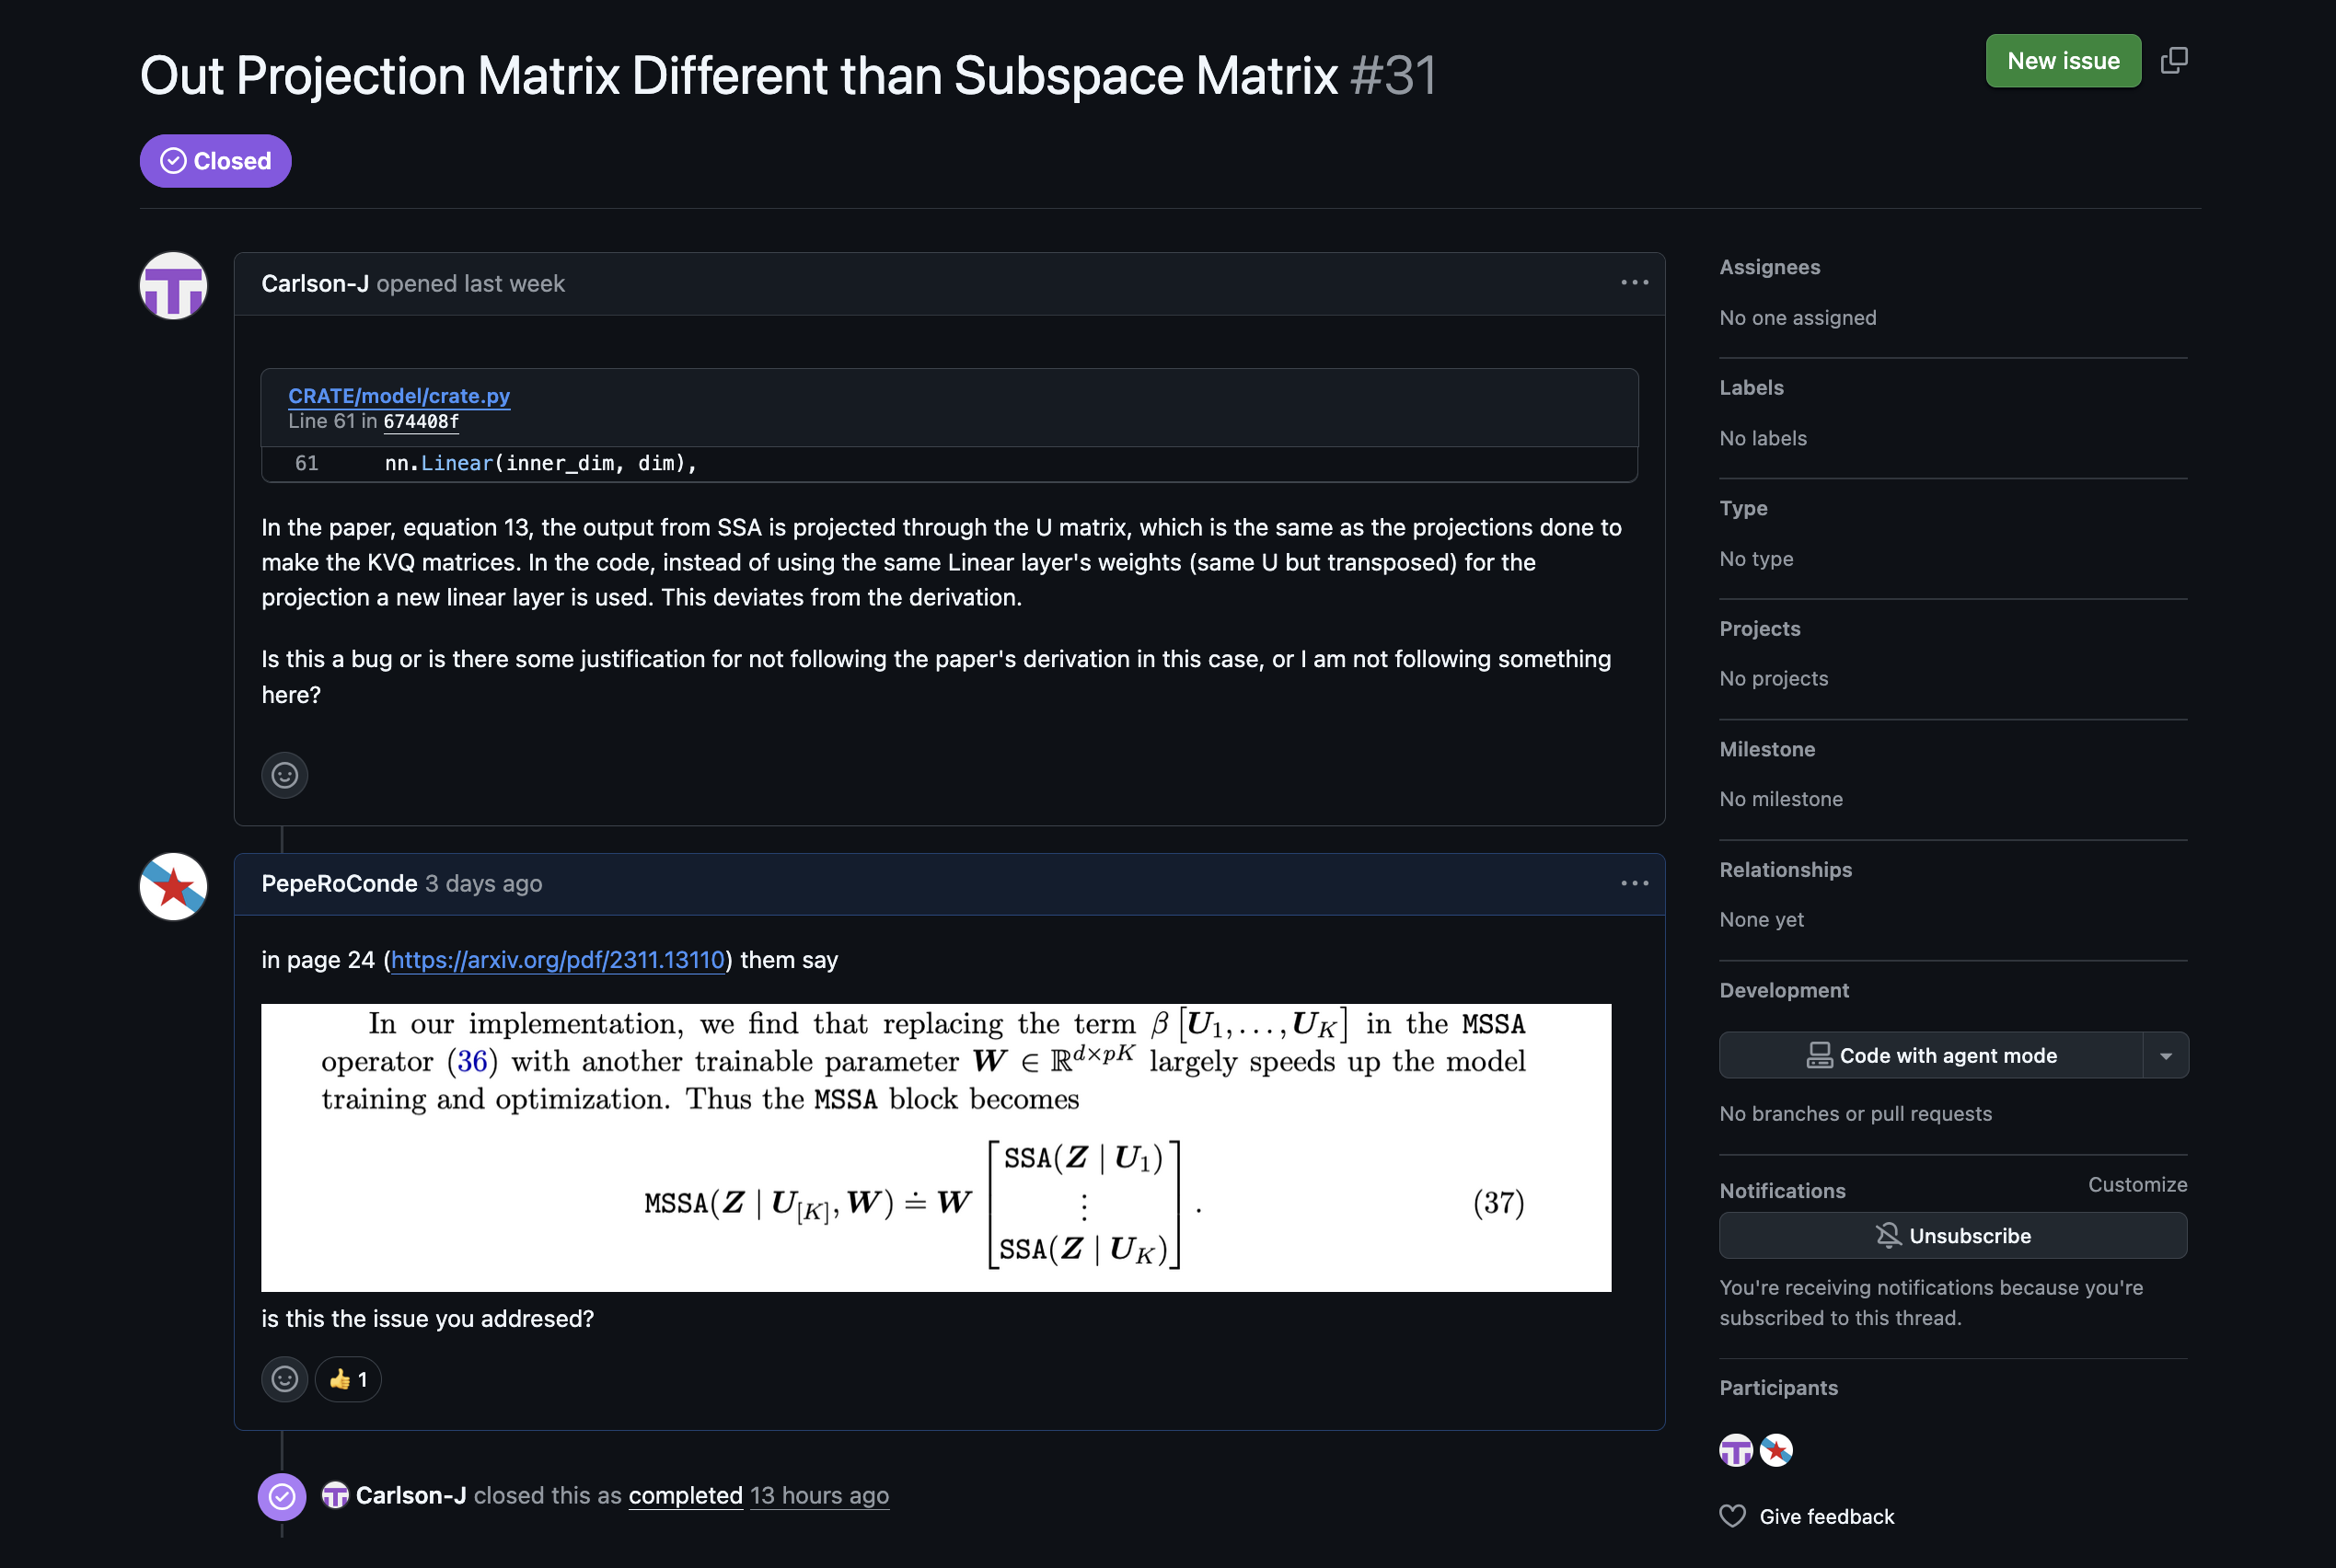
\includegraphics[width=\linewidth]{figs/issue.png}
\end{figure}

\end{document}
